\section{Type classes --- Functional design}
\subsection{Basics}

\begin{frame}
  \frametitle{by-value vs by-name}

  % TODO

\end{frame}

\begin{frame}
  \frametitle{lazy vs eager}

  % TODO

\end{frame}

\begin{frame}[fragile]
  \frametitle{Given/using (implicit values)}

  \texttt{using} clause defines a value to be injected by the compiler, based on the expected type among the \texttt{given} values

  \begin{example}
    \begin{lstlisting}
      given life: Int = 42
      def foo(using i: Int): Int = i
  
      val meaningOfLife1 = foo              // : Int = 42
      // rewritten as foo(life) by the compiler
      val meaningOfLife2 = foo(using life)  // : Int = 42
      // we can also explicitly pass the value
    \end{lstlisting}
  \end{example}
\end{frame}

\begin{frame}[fragile]
  \frametitle{Variance}

  \begin{definition}
    Describe the relation between generic types. Given a generic type \(\mathcal{F}\):
    \begin{description}
      \item[Invariant] \(\forall A,B\quad A \neq B \Leftrightarrow \mathcal{F}[A] \neq \mathcal{F}[B]\)
      \item[Covariant] \(\forall A,B\quad A <: B \Leftrightarrow \mathcal{F}[A] <: \mathcal{F}[B]\)
      \item[Contravariant] \(\forall A,B\quad A <: B \Leftrightarrow \mathcal{F}[B] <: \mathcal{F}[A]\)
    \end{description}
  \end{definition}

  \onslide<2->

  It allows a more flexible design, but has some constraints for type-safety. For a covariant type, we cannot use it's type param as method param type

  \begin{example}[Covariance constraint]
    \begin{lstlisting}
      class Foo[+A]:
        def foo[B >: A](x: B) = ??? // cannot use A as param type
    \end{lstlisting}
  \end{example}
\end{frame}

\subsection{Type classe}

\begin{frame}[fragile]
  \frametitle{Why type classes?}

  \begin{overprint}
    \onslide<1>
    \begin{example}[Inheritance]
      \begin{lstlisting}[gobble=8]
        trait Encoder      { def encode: String }
        trait Combiner[A] { def combine(a: A): String }
  
        abstract class Animal extends Encoder
          with Combiner[Animal]
  
        case class Cat() extends Animal:
          override def encode(): String
          override def combine(b: Animal): String
        case class Dog() extends Animal:
          override def encode(): String
          override def combine(b: Animal): String
      \end{lstlisting}
    \end{example}

    \onslide<2>

    \begin{example}[Composition]
      \begin{lstlisting}[gobble=8]
        trait Encoder[A]  { def encode (a: A): String }
        trait Combiner[A] { def combine(a: A, b: A): String }
    
        abstract class Animal(
          encoder: Encoder[Animal],
          combiner: Combiner[Animal]
        ):
          def encode = encoder.encode(this)
          def combine(b: Animal) = combiner.combine(this, b)
      \end{lstlisting}
    \end{example}

    \onslide<3>

    \begin{example}[Type class]
      \begin{lstlisting}[gobble=8]
        trait Encoder[-A] { def encode (a: A): String }
    
        abstract class Animal
    
        extension [A](a: A)(using encoder: Encoder[A])
          def encode: String = encoder.encode(a)
    
        given catEncoder: Encoder[Cat] with
          def encode(a: Cat) = "A cat"
    
        aCat.encode // "A cat"
        // rewritten as encode(aCat, catEncoder)
      \end{lstlisting}
    \end{example}
  \end{overprint}
\end{frame}

\begin{frame}
  \frametitle{Type class definition}

  \begin{enumerate}
    \item Define a trait (the behavior)
    \item Define your methods
    \item Define your trait instances
    \item (Optional) redefine methods as extension methods
  \end{enumerate}
\end{frame}

\begin{frame}[fragile]
  \frametitle{Exercices}

  \begin{enumerate}
    \item Define a type class \texttt{JsonEncoder} for a \texttt{case class Person} with a name, an age and an address
    \item Create a \texttt{JsonEncoder} for a \texttt{List[T]}
    \item Create a \texttt{JsonEncoder} for an \texttt{Option[T]}
    \item Try it with a \texttt{List[Option[Person]]}
  \end{enumerate}

  Given syntax help
  \begin{lstlisting}[gobble=4]
    given Type with
      // trait methods implementation
    given [A]: Type[A] with
      // trait methods implementation
    given [A](using otherGiven: OtherType[A]): Type[A] with
      // trait methods implementation
  \end{lstlisting}
\end{frame}

\begin{frame}[fragile]
  \frametitle{Exercices solution --- Part 1}

  \begin{lstlisting}[gobble=4]
    case class Person(...)
    
    // 1. TC definition
    trait JsonEncoder[-T]:
      def encode(t: T): String 

    // 3. TC instance for Person
    given JsonEncoder[Person] with
      def encode(person: Person): String = ???

    // 4. Redefine methods as extension methods
    extension [T](t: T)(using encoder: JsonEncoder[T])
      def toJson: String = encoder.encode(t)
  \end{lstlisting}

\end{frame}

\begin{frame}[fragile]
  \frametitle{Exercices solution --- Part 2}

  \begin{lstlisting}[gobble=4]
    // TC instance for List[T]
    given [T: JsonEncoder]: JsonEncoder[List[T]] with
      def encode(list: List[T]): String =
        list.map(_.toJson).mkString("[", ",", "]")

    // TC instance for Option[T]
    given [T: JsonEncoder]: JsonEncoder[Option[T]] with
      def encode(option: Option[T]): String =
        option.map(_.toJson).getOrElse("null")

    List(Some(lulu), None, Some(zozo)).toJson
    // : String = [
    //  {"name":"lulu",...}
    //  null
    //  {"name":"zozo",...}
    //]
  \end{lstlisting}
\end{frame}

\subsection{Common type classes}

\begin{frame}[fragile]
  \frametitle{Base types}

  \begin{definition}[Parser \& Result ADTs]
    \begin{lstlisting}
      sealed trait Parser[+A]:
        def parse(input: String): Result[A]
        protected def parse(input: String, index: Int): Result[A]
  
      sealed trait Result[+A]:
        def map[B](f: A => B): Result[B]
        def orElse[B](that: => Result[B]): Result[A | B]

      case class Success[+A](...) extends Result[A]
      case class Failure extends Result[Nothing]
    \end{lstlisting}
  \end{definition}
\end{frame}

% --------------------------------- Functors --------------------------------- %
\begin{frame}[fragile]
  \frametitle{Functor}

  \textbf{Problem} Need to transform a value inside any kind of (unrelated) data structure

  \begin{definition}[Functor]
    \begin{lstlisting}
      trait Functor[F[_]]:
        def map[A, B](fa: F[A])(f: A => B): F[B]
    \end{lstlisting}
  \end{definition}

  \onslide<2->
  \begin{itemize}
    \item Single abstraction for any \ul{generic} type
          \begin{itemize}
            \item Valid types: \texttt{Functor[List]}, \texttt{Functor[Option]}\dots
            \item Invalid types: \texttt{Functor[Int]}, \texttt{Functor[Person]}\dots
          \end{itemize}
    \item A bit more verbose (can be hidden with extension methods)
    \item Easy to switch from a data structure to another
  \end{itemize}
\end{frame}

\begin{frame}[fragile]
  \frametitle{Functor --- map implementation}

  \begin{enumerate}
    \item New concept \({\rightarrow}\) new case class
          \begin{itemize}
            \item Input: \texttt{Parser[A]} \& \texttt{A => B}
            \item Ouput: \texttt{Parser[B]}
          \end{itemize}
    \item No constructors, one combinator \& interpreter
  \end{enumerate}

  \onslide<2->

  \begin{lstlisting}[gobble=4]
    trait Parser[+A]:
      def map[B](f: A => B): Parser[B] = ParserMap(this, f)

    final case class ParserMap[A, B](
      source: Parser[A],
      f: A => B
    ) extends Parser[B]:
      override def parse(input: String, index: Int): Result[B] =
        source.parse(input, index).map(f)
  \end{lstlisting}
\end{frame}

% ---------------------------------- Monoids --------------------------------- %
\begin{frame}[fragile]
  \frametitle{Monoid}

  \textbf{Problem} Need to combine any kind of values

  \begin{definition}[Monoid]
    \begin{lstlisting}
      trait Monoid[A]:
        def empty: A
        def combine(a: A, b: A): A
    \end{lstlisting}
  \end{definition}

  \onslide<2->
  \begin{itemize}
    \item Single abstraction for \ul{any} type
    \item Can serve as a AND or OR operation
          \begin{itemize}
            \item AND:\ \texttt{combine(Parser1,Parser2) = Parser1 then Parser2}
            \item OR:\ \texttt{combine(Parser1,Parser2) = Parser1 orElse Parser2}
          \end{itemize}
    \item \texttt{Monoid}s without \texttt{empty} are called \texttt{Semigroup}s
  \end{itemize}
\end{frame}

\begin{frame}[fragile]
  \frametitle{Monoid --- orElse implementation}

  \begin{enumerate}
    \item New concept \({\rightarrow}\) new case class
          \begin{itemize}
            \item Input: \texttt{Parser[A]} \& \texttt{Parser[B]}
            \item Output: \texttt{Parser[A | B]}
          \end{itemize}
    \item No constructors, one combinator \& interpreter
  \end{enumerate}

  \onslide<2->
  \begin{lstlisting}[gobble=4]
    trait Parser[+A]:
      def orElse[B](that: => Parser[B]): Parser[A | B] =
        ParserOrElse(this, that)

    final class ParserOrElse[A, B](
      left: Parser[A],
      right: => Parser[B]
    ) extends Parser[A | B]:
      def parse(input: String, index: Int): Result[A | B] =
        left.parse(input, index)
            .orElse(right.parse(input, index))
  \end{lstlisting}
\end{frame}

% ------------------------------- Semigroupals ------------------------------- %
\begin{frame}[fragile]
  \frametitle{Semigroupal}

  \textbf{Problem} Need to operate on multiple values at once, without combining them (e.g. to instanciate a class)

  \begin{definition}[Semigroupal]
    \begin{lstlisting}
      trait Semigroupal[F[_]]:
        def product[A, B](fa: F[A], fb: F[B]): F[(A, B)]
    \end{lstlisting}
  \end{definition}

  \onslide<2->
  \begin{itemize}
    \item Single abstraction for \ul{generic} type
    \item Different from \texttt{Semigroup}
    \item Merge two values into one to use later
  \end{itemize}
\end{frame}

\begin{frame}[fragile]
  \frametitle{Semigroupal --- product implementation}

  \begin{enumerate}
    \item New concept \({\rightarrow}\) new case class
          \begin{itemize}
            \item Input: \texttt{Parser[A]} \& \texttt{Parser[B]}
            \item Output: \texttt{Parser[(A, B)]}
          \end{itemize}
    \item No constructors, one combinator \& interpreter
  \end{enumerate}

  \onslide<2->
  \begin{lstlisting}[gobble=4]
    trait Parser[+A]:
      def product[T >: A, B](that: Parser[B]): Parser[(T, B)] =
        ParserProduct(this, that)

    final case class ParserProduct[A, B](
      left: Parser[A],
      right: Parser[B]
    ) extends Parser[(A, B)]:
      def parse(input: String, index: Int): Result[(A, B)] =
        left.parse(input, index) match
          case fail: Failure => fail
          case Success(leftResult, _, offset) =>
            right.parse(input, offset).map((leftResult, _))
  \end{lstlisting}
\end{frame}

\begin{frame}[fragile]
  \frametitle{Semigroupal --- Monadic Combinations}

  When the container is a \texttt{Monad}, the \texttt{.product()} does a cartesian product (and bypasses `invalid' values like \texttt{None})

  \begin{example}[Monadic combination]
    \begin{lstlisting}
      Semigroupal[List].product(
        List(1, 2),
        List(4, 5),
      ) // List((1, 4), (1, 5), (2, 4), (2, 5))
      
      Semigroupal[Future].product(
        Future(throw new Exception),
        Future(throw new RuntimeException)
      ) // Failure(java.lang.Exception)
    \end{lstlisting}
  \end{example}
  /!\textbackslash{} With \texttt{List} \& \texttt{Future} being \texttt{Monad}s /!\textbackslash{}
\end{frame}

\begin{frame}[fragile]
  \frametitle{Semigroupal --- Applicative Combinations}

  When the container is not a \texttt{Monad}, the \texttt{.product()} keeps all the values (allows errors accumulation for instance)
  \begin{example}[Applicative combination]
    \begin{lstlisting}
      Semigroupal[???].product(
        Validated.invalid(List("Badness")),
        Validated.invalid(List("Fail"))
      ) // Invalid(List(Badness, Fail))

      Semigroupal[???].product(
        Validated.valid("Good"),
        Validated.valid(47),
      ) // Valid("Good", 47)
    \end{lstlisting}
  \end{example}
  /!\textbackslash{} With \texttt{Validated} \ul{not} being a \texttt{Monad} /!\textbackslash{}
\end{frame}

% ------------------------------- Applicatives ------------------------------- %
\begin{frame}[fragile]
  \frametitle{Applicative}

  \textbf{Problem} Need to apply a independent effects to value(s) of a container

  \begin{definition}[Applicative definition]
    \begin{lstlisting}
      trait Applicative[F[_]]:
        def pure[A](a: A): F[A]
        def ap[A, B](ff: F[A => B])(fa: F[A]): F[B]
    \end{lstlisting}
  \end{definition}

  \onslide<2->
  \begin{itemize}
    \item Single abstraction for \ul{generic} type
    \item Gives access to the \texttt{mapN} method, easier to manipulate than \texttt{product}
  \end{itemize}
\end{frame}

\begin{frame}[fragile]
  \frametitle{Applicative --- Example}

  Reminder: we cannot use \texttt{.flatMap}, it is not defined
  \begin{example}[Usage]
    \begin{lstlisting}
      val f: (Int, Int) => Int = _ + _
      val intList1 = List(5, 10, 15)
      val intList2 = List(0, 1)

      val adder = intList1.map(i1 => (i2: Int) => f(i1, i2))
      // List(i2 => f(5, c), i2 => f(10, c), i2 => f(15, c))
      adder.ap(intList2)
      // List(5, 6, 10, 11, 15, 16)
    \end{lstlisting}
  \end{example}
\end{frame}

% ---------------------------------- Monads ---------------------------------- %
\begin{frame}[fragile]
  \frametitle{Monad}

  \textbf{Problem} Need to chain operations on a same-kind container

  \begin{definition}[Monad definition]
    \begin{lstlisting}
      trait Monad[F[_]]:
        def flatMap[A, B](fa: F[A])(f: A => F[B]): F[B]
    \end{lstlisting}
  \end{definition}

  \onslide<2->
  \begin{itemize}
    \item Single abstraction for any \ul{generic} type
    \item Continue the chain only on success
    \item Stop the chain on first failure
  \end{itemize}
\end{frame}

\begin{frame}[fragile]
  \frametitle{Monad --- flatMap implementation}

  \begin{enumerate}
    \item New concept \({\rightarrow}\) new case class
          \begin{itemize}
            \item Input: \texttt{Parser[A]} \& \texttt{A => Parser[B]}
            \item Output: \texttt{Parser[B]}
          \end{itemize}
    \item No constructors, one combinator \& interpreter
  \end{enumerate}

  \onslide<2->
  \begin{lstlisting}[gobble=4]
    trait Parser[+A]:
      def flatMap[B](f: A => Parser[B]): Parser[B] =
        ParserFlatMap(this, f)

    final case class ParserFlatMap[A, B](
      source: Parser[A],
      f: A => Parser[B]
    ) extends Parser[B]:
      def parse(input: String, index: Int): Result[B] =
        source.parse(input, index) match
          case fail: Failure => fail
          case Success(result, input, offset) =>
            f(result).parse(input, offset)
  \end{lstlisting}

\end{frame}

% ---------------------------------- Summary --------------------------------- %
\begin{frame}
  \frametitle{Summary}

  \begin{description}
    \item[Functor] transform a value inside a container
    \item[Semigroupal] tuple values from any containers
    \item[Applicative] apply a independent effects to value(s) of a container
    \item[Monad] chain operations on same-kind containers
    \item[Monoid] combine values
  \end{description}
\end{frame}

\begin{frame}[fragile]
  \frametitle{Type class hierarchy}

  \begin{figure}[h]
    \centering
    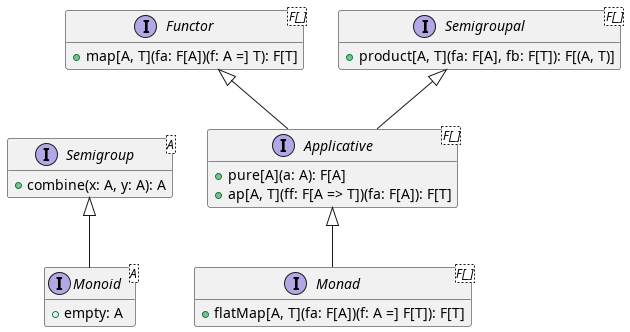
\includegraphics[width=0.9\linewidth]{img/tc-hierarchy.png}
    \caption{Hierarchy}
  \end{figure}
\end{frame}